\section{Relations and Functions}
\subsection{Ordered pairs}
In mathematics, relations and functions are usually defined in terms of ordered pairs. The key property the ordered pairs satisfied is as below
\begin{definition}{Ordered pairs}{}
    Basic property the ordered pairs should satisfy, which is also the axiomatic definition of ordered pairs
    \begin{equation*}
        \langle a,b \rangle = \langle c,d \rangle \iff a = b \land c = d
    \end{equation*}
\end{definition}
In 1921, Kazimierz Kuratowski give the construction of ordered pair based on ZF systems. 
\begin{definition}{Set based construction of ordered pairs}{}
    The \textbf{ordered pair}, with first component x and second component y, is the set defined by
    \begin{equation*}
        \langle x,y \rangle = \{\{x\}, \{x, y\}\}
    \end{equation*}
\end{definition}

\begin{lemma}{}{}
    Let $A$, $B$ be sets, there exists a unique set $\mathcal{D}$ s.t. for all $X$,
    \begin{equation*}
        X \in \mathcal{D} \iff X = \langle x,y \rangle \ \text{for some}\ x \in A \land y \in B.
    \end{equation*}
    or,
    \begin{equation*}
        X \in \mathcal{D} \iff (\exists x \in A)(\exists y \in B)(X = \langle x,y \rangle)
    \end{equation*}
    We shall denote $\mathcal{D}$ by $\{\langle x,y \rangle : x \in A \land y \in B\}$.
\end{lemma}

\begin{proof} 
    $X = \langle x,y \rangle \ \text{for some}\ x \in A \land y \in B \implies X = \{\{x\},\{x,y\}\} \in \mathcal{P}(\mathcal{P}(A \cup B) )$.\\
    The set $\mathcal{D}$ is uniquely defined by \Cref{class}.
\end{proof}

\begin{definition}{Cartesian product}{}
    Given sets $A$ and $B$, the \textbf{Cartesian product} $A \times B$ is defined to be the set
    \begin{equation*}
        A \times B = \{\langle x,y \rangle : x \in A \land y \in B\}
    \end{equation*}
    which is uniquely given by the above lemma.
\end{definition}

\subsection{Relations}
\begin{definition}{Relations}{}
    A \textbf{Relation} $R$ is a set of orded pairs. In other words, for all $x$,
    \begin{equation*}
        x \in R \iff x = \langle a,b \rangle \ \text{for some}\ a\ \text{and}\ b.
    \end{equation*}
\end{definition}

\begin{definition}{}{}
    Let $A$ and $B$ be sets. 
    \begin{enumerate}

        \item A \textbf{relation from $A$ to $B$} is a subset of $A \times B$, or $R \subseteq A \times B$. 
        \item A \textbf{relation on $A$} is a subset of $A \times A$, or $R \subseteq A \times A$. 
    \end{enumerate}
\end{definition}

\begin{remarks}
    by subset axiom, given a formula $\varphi(x,y)$, and sets $A$ and $B$, we can construct a relation R,
    \begin{equation*}
        R = \{\langle x,y \rangle \in A \times B : \varphi(x,y)\}
    \end{equation*}
\end{remarks}

\begin{lemma}{}{}
    Let $R$ be a relation and $A = \cup \cup R$. Then $R \subseteq A \times A$.
\end{lemma}

We conclude that every relation can be viewed as a relation on one set.

\begin{definition}{}{}
    Let R is a relation:
    \begin{enumerate}

        \item The \textbf{domain} of $R$: $dom{R} = \{x : \exists y (\langle x,y \rangle \in R)\}$.
        \item The \textbf{range} of $R$: $ran{R} = \{y : \exists x (\langle x,y \rangle \in R)\}$.

    \end{enumerate}
\end{definition}

\begin{remarks}
    we have concluded that $x, y \in \cup \cup R$, hence the domain and range of relation $R$ are proofed to to be sets by \Cref{class}.
\end{remarks}

\begin{definition}{Operations on relations}{}
    Let $R$ and $S$ be relations, and given set $A$
    \begin{enumerate}

        \item the \textbf{inverse} of $R$ is the relation
        \begin{equation*}
            R^{-1} = \{\langle y,x \rangle : \langle x,y \rangle \in R\}
        \end{equation*}
        or
        \begin{equation*}
            \langle y,x \rangle \in R^{-1} \iff \langle x,y \rangle \in R
        \end{equation*}
        \item the \textbf{restriction} of $R$ to $A$ is the relation
        \begin{equation*}
            R \vert_{A} = \{\langle x,y \rangle : \langle x,y \rangle \in R \land x \in A\}
        \end{equation*}
        \item the \textbf{image} of $A$ under $R$ is the set
        \begin{equation*}
            R[A] = \{y : \exists x \in A (\langle x,y \rangle \in R)\}
        \end{equation*}
        \item the \textbf{inverse image} of $A$ under $R$ is the set
        \begin{equation*}
            R^{-1}[A] = \{x : \exists y \in A(\langle x,y \rangle \in R)\}
        \end{equation*}
        \item the \textbf{composition} of $R$ and $S$ is the relation
        \begin{equation*}
            R \circ S = \{\langle x,z \rangle : \exists y (\langle x,y \rangle \in S \land \langle y,z \rangle \in R)\}
        \end{equation*}
    \end{enumerate}
\end{definition}

\begin{proposition}{}{}
    Let $R$,$S$ and $T$ be relations, then
    \begin{enumerate}

        \item $dom R^{-1} = ran R$
        \item $ran R^{-1} = dom R$
        \item $(R^{-1})^{-1} = R$ 
        \item $(R \circ S)^{-1} = S^{-1} \circ R^{-1}$
        \item $R \circ (S \circ T) = (R \circ S) \circ T$

    \end{enumerate}
\end{proposition}

\begin{proposition}{}{}
    Suppose $\mathcal{F}$ is a collections of sets, and R is a relation
    \begin{enumerate}

        \item $R[\bigcup \mathcal{F}] = \bigcup \{R[F] : F \in \mathcal{F}\}$
        \item $R[\bigcap \mathcal{F}] \subseteq \bigcap \{R[F] : F \in \mathcal{F}\}$ ($\mathcal{F}$ is nonempty)

    \end{enumerate}
\end{proposition}
The above proposition proclaim that the image of a union is the union of the images,” whereas “the image of an intersection is a subset of the intersection of the images.

\begin{definition}{Single-rooted}{}
    A relation $R$ is \textbf{single-rooted} if for every $y \in ran R$, there is exactly one $x$ s.t. $\langle x,y \rangle \in R$. In other words
    \begin{equation*}
        \langle x,z \rangle \in R \land \langle y,z \rangle \in R \implies x = y
    \end{equation*}
\end{definition}

\begin{corollary}{}{}
    Let $R$ be a single-rooted relation. Suppose that A and B are sets and $\mathcal{F}$ is a nonempty collection.
    \begin{enumerate}

        \item $R[\bigcap \mathcal{F}] = \bigcap \{R[F] : F \in \mathcal{F}\}$ 
        \item $R[A \setminus B] = R[A] \setminus R[B]$

    \end{enumerate}
\end{corollary}

\subsubsection{Equivalence relations}
Let $R$ be a relation. If $\langle x,y \rangle \in R$, we shall say that x is related to y, sometimes it is also written as $xRy$. 

\begin{definition}{Equivalence relation}{}
    Let $\sim$ be a relation on $A$. For any $x$, $y$ and $z$ in $A$.
    \begin{enumerate}

        \item \textbf{reflexive}: $x \sim x$
        \item \textbf{symmetric}: $x \sim y \implies y \sim x$
        \item \textbf{transitive}: $x \sim y \land y \sim z \implies x \sim z$

    \end{enumerate}
    A relation is called a \textbf{equivalence relation} on A, if it is reflexive, symmetric and transitive.
\end{definition}

\begin{remarks}
    \begin{enumerate}

        \item The relation is \textit{reflexive} if every element in the set A is related to itself.
        \item The relation is \textit{symmetric} if whenever x is related to y, then y is related to x.
        \item The relation is \textit{transitive} if whenever x is related to y and y is related to z, then x is also related to z.

    \end{enumerate}
\end{remarks}

\begin{definition}{Partition}{}
    Let $A$ be a set. Let $\mathcal{P}$ be a collection of nonempty subsets of $A$. We say that $\mathcal{P}$ is a \textbf{partition} of $A$ if the following two conditions hold:
    \begin{enumerate}

        \item for every $x \in A$, there is a $P \in \mathcal{P}$ s.t. $x \in P$.
        \item for any $P$ and $Q$ in $\mathcal{P}$, if $P \neq Q$, then $P \cap Q = \emptyset$. Sometimes we call that sets in $\mathcal{P}$ are \textbf{pairwise disjoint}.    

    \end{enumerate}
\end{definition}
    
\begin{definition}{Equivalence class}{}
    Let $\sim$ be an equivalence relation on $A$, and $a$ be an element of $A$. The \textbf{equivalence class} of $a$ is the set consists of all elements of $A$ which are related to $a$. We denote it as
    \begin{equation*}
        [a] = \{x \in A: x \sim a\}
    \end{equation*}
\end{definition}

\begin{theorem}{}{}
    Let $\sim$ be an equivalence relation of $A$. For any $a$, $b \in A$,
    \begin{equation*}
        a \sim b \iff [a] = [b]
    \end{equation*}
\end{theorem}

\begin{proof}
    (\implies )
    \begin{align*}
        x \in [a] &\implies x \sim a\\
        &\implies x \sim a \land a \sim b \implies x \sim b\\
        &\implies x \in [b]\\
    \end{align*}
    \begin{align*}
        x \in [b] &\implies x \sim b\\
        &\implies x \sim b \land b \sim a \implies x \sim a\\
        &\implies x \in [a]\\
        &\implies [a] = [b]\\
    \end{align*}
    ($\Leftarrow $ )
    \begin{align*}
        [a] = [b] &\implies a \in [b]\\
        &\implies a \sim b
    \end{align*}
\end{proof}

\begin{corollary}{}{}
    Let $\sim$ be an equivalence relation of $A$. For any $a$, $b \in A$,
    \begin{equation*}
        a \in [b] \iff [a] = [b]
    \end{equation*}
\end{corollary}

\begin{theorem}{Fundamental Theorem of Equivalence Relation 1}{}
    Let $\sim$ be an equivalence relation on $A$. Then the collection $A/\sim = \{[a]: a \in A\} $ is a partition of A. Sometimes we call $A/\sim$ the \textbf{quotient set induced by} $\sim$.
\end{theorem}

\begin{proof}
    Firstly, we proof the existence of the collection $A/\sim$. Obviously, The collection can be written as $\{X: \exists a \in A (X = [a])\}$, which implies that $X \in \mathcal{P}(A) $. By \Cref{class}, $A/\sim$ is a set.\\
    Then we proof $A/\sim$ is a partition of A.
    \begin{enumerate}

        \item for every $a \in A$, we can find $[a] \in A/\sim$ s.t. $a \in [a]$.
        \item Let $[a]$, $[b] \in A/\sim$, and  $[a] \neq [b]$. Assume $[a] \cap [b] \neq \emptyset\\$
        \begin{align*}
            &[a] \cap [b] \neq \emptyset \\
            &\implies x \in [a] \land x \in [b]\\
            &\implies [x] = [a] \land [x] = [b]\\
            &\implies [a] = [b] 
        \end{align*} 

        Which is a contradiction.

    \end{enumerate}
\end{proof}

\begin{theorem}{Fundamental Theorem of Equivalence Relation 2}{}
    Let $\mathcal{P}$ be a partition of a set $A$. Then there is an equivalence relation $\sim$ on $A$ defined as follows: 
    \begin{equation*}
        x \sim y \iff x \in P \land y \in P \ \text{for some}\ P \in \mathcal{P}.
    \end{equation*}
\end{theorem}

\begin{proof}
    We just proof the relation $\sim$ satisfy reflexive, symmetric and transitive properties.
    \begin{enumerate}

        \item reflexive:
        \begin{equation*}
            \forall x \in A \exists P \in \mathcal{P} (x \in P) \implies \forall x \in A (x \sim x)
        \end{equation*}
        \item symmetric: trivial.
        \item transitive:
        \begin{align*}
            &x \sim y \land y \sim z\\
            &\implies (x,y \in P \ \text{for some}\ P \in \mathcal{P})\land (y,z \in S \ \text{for some}\ S \in \mathcal{P})\\
            &\implies y \in P \land y \in S\\
            &\implies P = S\\
            &\implies x,z \in P \ \text{for some}\ P \in \mathcal{P}\\
            &\implies x \sim z
        \end{align*}

    \end{enumerate}
\end{proof}

\begin{examples}
    There is an equivalence relation on $\mathbb{Z}$, defined by
    \begin{equation*}
        m \sim n \iff 3 | (m - n)
    \end{equation*}
    We get the equivalence class $[n]$:
    \begin{equation*}
        [n] = \{m \in \mathbb{Z}: m \sim n\} = \{3k+n: k \in \mathbb{Z}\}
    \end{equation*}
    \begin{align*}
        [0] &= \{...-3,0,3,6\}\\
        [1] &= \{...-2,1,4,7\}\\
        [2] &= \{...-1,2,5,8\}\\
    \end{align*}
    Finally, we can the quotient set:
    \begin{equation*}
        \mathbb{Z}/\sim = \{[0],[1],[2]\}
    \end{equation*}
\end{examples}

\subsubsection{Order relations}

\begin{definition}{Partial order}{}
    Let $\preceq$ be a relation on $A$. For any $x$, $y$ and $z$ in $A$.
    \begin{enumerate}

        \item \textbf{reflexive}: $x \preceq x$
        \item \textbf{antisymmetric}: $x \preceq y \land y \preceq x \implies x = y$
        \item \textbf{transitive}: $x \preceq y \land y \preceq z \implies x \preceq z$

    \end{enumerate}
    A relation is called a \textbf{partial order} on A, if it is reflexive, antisymmetric and transitive. We shall say that order pairs $(A,\preceq)$ is a \textbf{poset}.
\end{definition}

\begin{examples}
    the power set of $\{x,y,z\}$ under the inclusion relation is a poset.
\end{examples}

\begin{figure}[h]
    \centering
    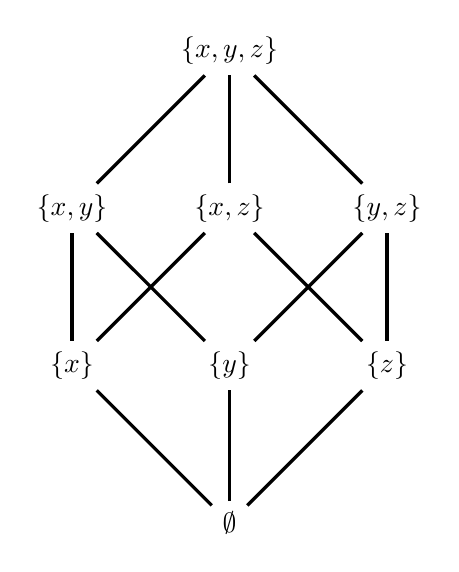
\begin{tikzpicture}[scale=2, very thick]
        % Nodes (subsets of {x, y, z})
        \node (xyz) at (0,2.5) {$\{x,y,z\}$};
        \node (xy) at (-1,1.5) {$\{x,y\}$};
        \node (xz) at (0,1.5) {$\{x,z\}$};
        \node (yz) at (1,1.5) {$\{y,z\}$};
        \node (x) at (-1,0.5) {$\{x\}$};
        \node (y) at (0,0.5) {$\{y\}$};
        \node (z) at (1,0.5) {$\{z\}$};
        \node (empty) at (0,-0.5) {$\emptyset$};
        
        % Edges (showing the subset relation)
        \draw (empty) -- (x);
        \draw (empty) -- (y);
        \draw (empty) -- (z);
        \draw (x) -- (xy);
        \draw (x) -- (xz);
        \draw (y) -- (xy);
        \draw (y) -- (yz);
        \draw (z) -- (xz);
        \draw (z) -- (yz);
        \draw (xy) -- (xyz);
        \draw (xz) -- (xyz);
        \draw (yz) -- (xyz);
    \end{tikzpicture}
    \caption{Hasse diagram of all subsets of the set $\{x,y,z\}$ with the subset relation.}
    \label{fig:hasse-diagram}
\end{figure}

\newpage

\begin{definition}{Total order}{}
    Let $(A,\preceq)$ be a poset, if relation $\preceq$ satisfy that for any $x,y \in A$,
    \begin{equation*}
        x \preceq y \lor y \preceq x
    \end{equation*}
    then relation $\preceq$ is \textbf{totally order} on $A$ and we call that $A$ is a \textbf{toset}.
\end{definition}

\begin{remarks}
    sometimes we call that $x$ and $y$ are comparable if either $x \preceq y$ or $y \preceq x$.
\end{remarks}
\begin{definition}{Strict order corresponding to $\preceq$}{}
    Let $(A,\preceq)$ be a poset, for any $x,y \in A$, we define
    \begin{equation*}
        x \prec y \iff  x \preceq y \land x \neq y
    \end{equation*}
    The relation $\prec$ on $A$ shall be called as the \textbf{strict order} corresponding to $\preceq$.
\end{definition}

\begin{remarks}
    strict order is obviously not partial order, because it is not reflexive. And $\succeq$ is just the inverse of $\preceq$. That is
    \begin{equation*}
        \succeq \ = \ \preceq^{-1}
    \end{equation*}
\end{remarks}

\begin{definition}{Maximal and Minimal}{}
    Let $(A,\preceq)$ be a poset, 
        \begin{enumerate}

            \item a element $m \in A$ is called a \textbf{maximal} iff $m \nprec x \ \text{for all}\ x \in A$.
            \item a element $n \in A$ is called a \textbf{minimal} iff $x \nprec n \ \text{for all}\ x \in A$.

        \end{enumerate}

    That is to say there is no element in $A$ which is larger than $m$, and smaller than $n$.
\end{definition}

\begin{remarks}
    equivalently, the definitions can be reclaimed as 
    \begin{enumerate}

        \item $\forall x \in A (m \preceq x \implies m = x)$
        \item $\forall x \in A (x \preceq n \implies x = n)$

    \end{enumerate}
\end{remarks}

\begin{examples}
    The Diagram below shows that minimal and maximal may not be unique in the set.
\end{examples}

\begin{figure}[ht]
    \centering
    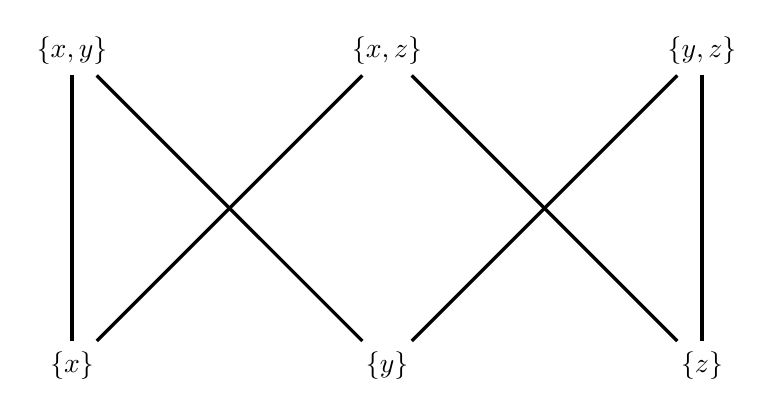
\begin{tikzpicture}[scale=2.0, very thick]
      % Define the nodes
      \node (xy) at (0,2) {$\{x, y\}$};
      \node (xz) at (2,2) {$\{x, z\}$};
      \node (yz) at (4,2) {$\{y, z\}$};
      
      \node (x) at (0,0) {$\{x\}$};
      \node (y) at (2,0) {$\{y\}$};
      \node (z) at (4,0) {$\{z\}$};

      % Draw the edges
      \draw (x) -- (xy);
      \draw (y) -- (xy);
      \draw (x) -- (xz);
      \draw (z) -- (xz);
      \draw (y) -- (yz);
      \draw (z) -- (yz);
    \end{tikzpicture}
    \caption{Hasse diagram of all subsets of \{x, y, z\} except the empty set and \{x, y, z\} itself.}
\end{figure}

\begin{definition}{Greatest and Least}{}
    Let $(A,\preceq)$ be a poset, 
    \begin{enumerate}

            \item a element $m \in A$ is called a \textbf{greatest} iff $x \preceq m \ \text{for all}\ x \in A$.
            \item a element $n \in A$ is called a \textbf{least} iff $n \preceq x \ \text{for all}\ x \in A$.

    \end{enumerate}

\end{definition}

\begin{remarks}
    If the greatest and least exists, then they must be unique, the proof is trivial.
\end{remarks}

\begin{proposition}{}{}
    Let $(A,\preceq)$ be a poset, if the greatest $m$ exists, then $m$ is also the maximal. In same way, if the least $n$ exists, then $n$ is also the minimal.
\end{proposition}

\begin{proof}
    We just proof the first claim. Let $m$ be the greatest element.
    For any $x \in A$.
    \begin{align*}
        &m \preceq x\\
        &\implies m \preceq x \land x \preceq m\\
        &\implies m = x
    \end{align*}
\end{proof}

\begin{theorem}{}{}
    Let $(A,\preceq)$ be a toset. If the maximal exists, then it is also the greatest element and unique. 
    If the minimal exists, then it is also the least element and unique.
\end{theorem}

\begin{proof}
    We proof the first claim. Let $m$ be the maximal. For any $x \in A$,
    \begin{align*}
        &m \preceq x \implies m = x\\
        &m \preceq x \lor x \preceq m \ \text{(definition of toset)}\\
        &\implies m = x \lor x \preceq m \ \text{and}\  m = x \implies x \preceq m\\
        &\implies x \preceq m 
    \end{align*}
    The uniqueness is due to the uniqueness of the greatest element.
\end{proof}

\subsection{Functions}

\begin{definition}{Single-valued}{}
    A relation $R$ is \textbf{Single-valued} if for every $x \in dom R$, there is exactly one $y$ s.t. $\langle x,y \rangle \in R$. In other words
    \begin{equation*}
        \langle x,y \rangle \in R \land \langle x,z \rangle \in R \implies y = z
    \end{equation*}
\end{definition}

\begin{definition}{Functions}{}
    A \textbf{function} is a single-valued relation.
\end{definition}

\begin{definition}{Functions from A to B}{}
    Let $A$ and $B$ be sets, and $F$ be a relation from $A$ to $B$. Then $F$ is 
    said to be a \textbf{function from $A$ to $B$} if following conditions holds:
    \begin{enumerate}

        \item $dom(F) = A$.
        \item $F$ is single-valued.

    \end{enumerate}
    The $A$ is \textbf{domain} of $F$, and $B$ is the \textbf{codomain} of $F$.\\
    We usually call that a function $F$ from $A$ to $B$ is a subset of $A \times B$ s.t. for each $x \in A$, there is exactly one $y \in B$ so that $\langle x,y \rangle \in F$.
\end{definition}

We write \underline{$F : A \to B$ to denote that $F$ is a function from the set $A$ to the set $B$.} Thus, for each $x \in A$, there is exactly one $y \in B$ such that $\langle x, y \rangle \in F$. This unique $y$ is called \underline{“the value of $F$ at $x$” and is denoted by $F(x)$.} Therefore, $\langle x, y \rangle \in F$ if and only if $F(x) = y$.
Moreover, one can also say that \underline{the function $F$ maps $x$ to $F(x)$, denoted by $x \mapsto F(x)$.} 

\begin{examples}
    Arrow diagram with domain as a red ellipse and codomain as a green ellipse representing the function \( F: A \to B \) defined by \( F = \{\langle a, 3 \rangle, \langle b, 5 \rangle, \langle c, 1 \rangle, \langle d, 3 \rangle\} \)
\end{examples}

\begin{figure}[htbp]
    \centering
    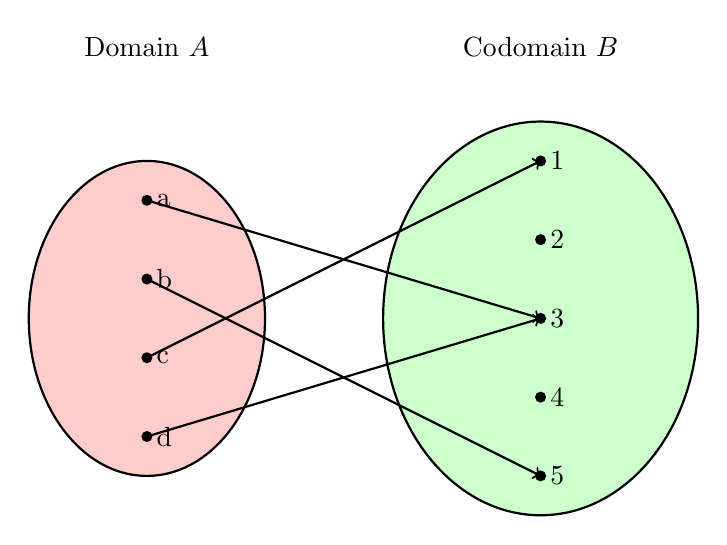
\begin{tikzpicture}

    % Red ellipse for domain A and green ellipse for codomain B
    \draw[thick, fill=red!20] (-2, 2.5) ellipse [x radius=1.5, y radius=2] node[above=3.2cm] {Domain \( A \)};
    \draw[thick, fill=green!20] (3, 2.5) ellipse [x radius=2, y radius=2.5] node[above=3.2cm] {Codomain \( B \)};

    % Black dots for elements of A inside the red ellipse
    \fill[black] (-2,4) circle (2pt) node[right] {a};
    \fill[black] (-2,3) circle (2pt) node[right] {b};
    \fill[black] (-2,2) circle (2pt) node[right] {c};
    \fill[black] (-2,1) circle (2pt) node[right] {d};

    % Black dots for elements of B inside the green ellipse
    \fill[black] (3,4.5) circle (2pt) node[right] {1};
    \fill[black] (3,3.5) circle (2pt) node[right] {2};
    \fill[black] (3,2.5) circle (2pt) node[right] {3};
    \fill[black] (3,1.5) circle (2pt) node[right] {4};
    \fill[black] (3,0.5) circle (2pt) node[right] {5};

    % Thicker arrows representing the function
    \draw[thick,->] (-2,4) -- (3,2.5); % a -> 3
    \draw[thick,->] (-2,3) -- (3,0.5); % b -> 5
    \draw[thick,->] (-2,2) -- (3,4.5); % c -> 1
    \draw[thick,->] (-2,1) -- (3,2.5); % d -> 3

    \end{tikzpicture}
    \caption{Arrow diagram representing the function \( F: A \to B \) defined by \( F = \{\langle a, 3 \rangle, \langle b, 5 \rangle, \langle c, 1 \rangle, \langle d, 3 \rangle\} \)}
    \label{fig:arrow-diagram}
\end{figure}

\begin{example}
    $F(x) = 2x^3 + 1,\ \text{for all } x \in \mathbb{R}.$ is a function, we can rewrite it in formal way:
    \begin{equation*}
        F = \{\langle x,y \rangle \in \mathbb{R}\times \mathbb{R}: y = 2 x^{3} + 1\}
    \end{equation*}
\end{example}

\begin{figure}[h]
    \centering
    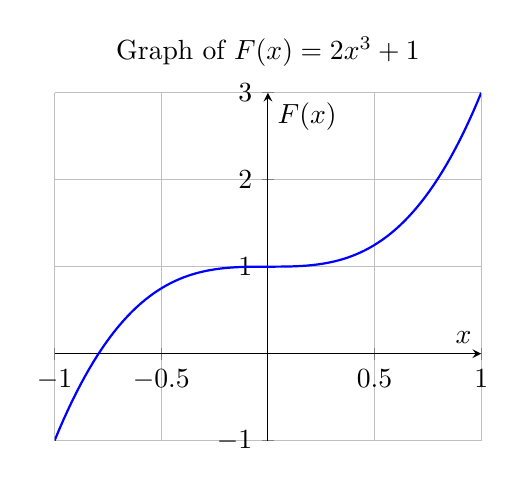
\begin{tikzpicture}
        \begin{axis}[
            axis lines = middle,
            xlabel = \( x \),
            ylabel = \( F(x) \),
            domain = -1:1,
            samples = 100,
            grid = both,
            title = {Graph of \( F(x) = 2x^3 + 1 \)},
            width = 7cm,
            height = 6cm
            ]
            \addplot[
                blue,
                thick
            ]
            {2*x^3 + 1};
        \end{axis}
    \end{tikzpicture}
    \caption{Graph of the function \( F(x) = 2x^3 + 1 \) for all \( x \in \mathbb{R} \)}
    \label{fig:graph}
\end{figure}

\begin{theorem}{}{}
    Let $F$ and $G$ be functions with common domain s.t. $domF = domG$. Then
    \[
        F = G \iff F(x) = F(y) \ \text{for all}\ x, y \in domF.
    \]
\end{theorem}

\begin{definition}{}{}
Let $A$ and $B$ be sets. The set of all functions from $A$ to $B$, denoted by $B^A$, is defined by
\[
B^A = \{ F : F : A \to B \}.
\]
\end{definition}

\begin{remarks}
    The existence of $B^{A}$ is guaranteed by \Cref{class} due to that $F \in \mathcal{P}(A \times B) $.
\end{remarks}

\begin{examples}
    The empty function is the function whose domain is empty set. For every set $B$, there is a unique empty function $f: \varnothing \to B$. Due to $f \subseteq \varnothing \times B$, which is just empty set,  the empty function is just empty set.
    \[
        B^{\varnothing} = \{\varnothing\}
    \]
    and 
    \[
        \varnothing^A = \varnothing
    \]
\end{examples}

\begin{definition}{Operations on functions}{}
    Let $F$ and $G$ be functions, and given set $A$
    \begin{enumerate}

        \item the \textbf{inverse} of $F$ is the \underline{relation} 
        \begin{equation*}
            F^{-1} = \{\langle y,x \rangle : F(x) = y\}
        \end{equation*}
        or
        \begin{equation*}
            \langle y,x \rangle \in F^{-1} \iff F(x) = y
        \end{equation*}
        \item the \textbf{restriction} of $F$ to $A$ is the function
        \begin{equation*}
            F \vert_{A} = \{\langle x,y \rangle : F(x) = y \land x \in A\}
        \end{equation*}
        \item the \textbf{image} of $A$ under $F$ is the set
        \begin{equation*}
            F[A] = \{y : \exists x \in A (F(x) = y)\} = \{F(x): x \in A\}
        \end{equation*}
        \item the \textbf{inverse image} of $B$ under $F$ is the set
        \begin{equation*}
            F^{-1}[B] = \{x : \exists y \in B(F(x) = y)\} = \{x : F(x) \in B\}
        \end{equation*}
        \item the \textbf{composition} of $F$ and $G$ is the function
        \begin{equation*}
            F \circ G = \{\langle x,z \rangle : \exists y (G(x)=y \land F(y)=z)\}
        \end{equation*}
    \end{enumerate}
\end{definition}

\subsubsection{One-to-one functions}
If a function has no repeated values, then we will say that the function is one-to-one.
For example:

\begin{figure}[h]
    \centering
    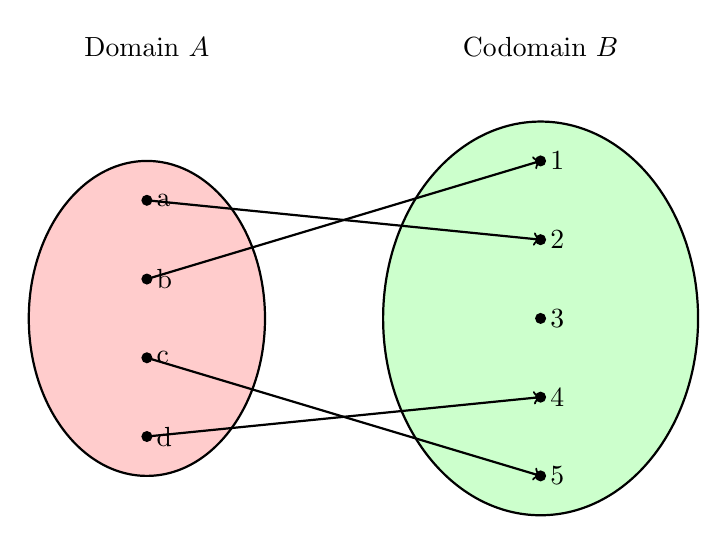
\begin{tikzpicture}

    % Red ellipse for domain A and green ellipse for codomain B
    \draw[thick, fill=red!20] (-2, 2.5) ellipse [x radius=1.5, y radius=2] node[above=3.2cm] {Domain \( A \)};
    \draw[thick, fill=green!20] (3, 2.5) ellipse [x radius=2, y radius=2.5] node[above=3.2cm] {Codomain \( B \)};

    % Black dots for elements of A inside the red ellipse
    \fill[black] (-2,4) circle (2pt) node[right] {a};
    \fill[black] (-2,3) circle (2pt) node[right] {b};
    \fill[black] (-2,2) circle (2pt) node[right] {c};
    \fill[black] (-2,1) circle (2pt) node[right] {d};

    % Black dots for elements of B inside the green ellipse
    \fill[black] (3,4.5) circle (2pt) node[right] {1};
    \fill[black] (3,3.5) circle (2pt) node[right] {2};
    \fill[black] (3,2.5) circle (2pt) node[right] {3};
    \fill[black] (3,1.5) circle (2pt) node[right] {4};
    \fill[black] (3,0.5) circle (2pt) node[right] {5};

    % Thicker arrows representing the function
    \draw[thick,->] (-2,4) -- (3,3.5); % a -> 2
    \draw[thick,->] (-2,3) -- (3,4.5); % b -> 1
    \draw[thick,->] (-2,2) -- (3,0.5); % c -> 5
    \draw[thick,->] (-2,1) -- (3,1.5); % d -> 4

    \end{tikzpicture}
    \caption{Arrow diagram representing the function \( F: A \to B \) defined by \( F = \{\langle a, 2 \rangle, \langle b, 1 \rangle, \langle c, 5 \rangle, \langle d, 4 \rangle\} \)}
    \label{fig:injection}
\end{figure}

\begin{definition}{Injection}{}
    A function $F$ is said to be \textbf{one-to-one}, or \textbf{injection} iff for any $x, y \in domF$
    \begin{equation*}
        F(x) = F(y) \implies x = y
    \end{equation*}
    In other words, distinct elements are mapped to distinct elements. 
\end{definition}

\begin{lemma}{}{}
    A function $F$ is one-one iff it is single-rooted.
\end{lemma}

\begin{theorem}{}{}
    Let $F$ be a relation. 
    \begin{enumerate}

        \item Then $F^{-1}$ is a function iff $F$ is single-rooted.
        \item Then $F$ is a function iff $F^{-1}$ is single-rooted.

    \end{enumerate}
\end{theorem}

\begin{proof}
    ($\implies $)\\
    To proof $F$ is single-rooted, Suppose
    \begin{align*}
        &\langle x,z \rangle \in F \land \langle y,z \rangle \in F\\
        &\implies \langle z,x \rangle \in F^{-1} \land \langle z,y \rangle \in F^{-1} \\
        &\implies x = y
    \end{align*}

    ($\Leftarrow $)
    To proof $F^{-1}$ is single-valued, Suppose
    \begin{align*}
        &\langle z,x\rangle \in F^{-1} \land \langle z,y \rangle \in F^{-1}\\
        &\implies \langle x,z \rangle \in F \land \langle y,z \rangle \in F\\
        &\implies x = y
    \end{align*}
\end{proof}

\begin{corollary}{}{}
    $F$ is a one-one function, $F^{-1}$ is also a one-one function.
\end{corollary}

\begin{proof}
    Firstly, $F$ is single-rooted implies $F^{-1}$ is a function. Then 
    $F$ is a function implies $F^{-1}$ is single-rooted. So $F^{-1}$ is one-one.
\end{proof}

\begin{theorem}{}{}
    Let $F$ be a one-one function.
    \begin{enumerate}

        \item $(F^{-1} \circ F)(x) = x$ for all $x \in domF$
        \item $(F \circ F^{-1})(y) = y$ for all $y \in ranF$

    \end{enumerate}
\end{theorem}

\begin{proof}
    for every $x \in domF$, there exits $y \in ranF$ s.t. $F(x) = y$.
    \begin{equation*}
        F^{-1} \circ F(x) = F^{-1}(F(x))
    \end{equation*}
\end{proof}

\begin{definition}{Surjection}{}
    A function $F : A \to B$ maps A \textbf{onto} B, or \textbf{surjection} iff $ranF = B$, that is for any $y \in B$
    \begin{equation*}
        \exists x \in A(F(x) = y)
    \end{equation*}
\end{definition}

\begin{figure}[h]
    \centering
    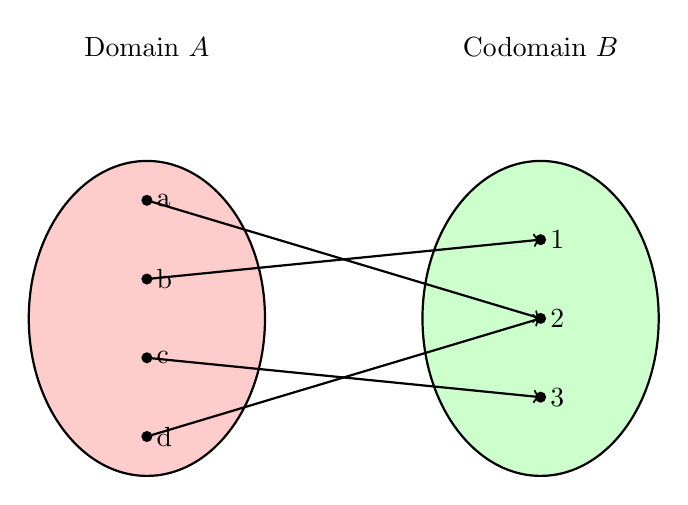
\begin{tikzpicture}

    % Red ellipse for domain A and green ellipse for codomain B
    \draw[thick, fill=red!20] (-2, 2.5) ellipse [x radius=1.5, y radius=2] node[above=3.2cm] {Domain \( A \)};
    \draw[thick, fill=green!20] (3, 2.5) ellipse [x radius=1.5, y radius=2] node[above=3.2cm] {Codomain \( B \)};

    % Black dots for elements of A inside the red ellipse
    \fill[black] (-2,4) circle (2pt) node[right] {a};
    \fill[black] (-2,3) circle (2pt) node[right] {b};
    \fill[black] (-2,2) circle (2pt) node[right] {c};
    \fill[black] (-2,1) circle (2pt) node[right] {d};

    % Black dots for elements of B inside the green ellipse
    \fill[black] (3,3.5) circle (2pt) node[right] {1};
    \fill[black] (3,2.5) circle (2pt) node[right] {2};
    \fill[black] (3,1.5) circle (2pt) node[right] {3};

    % Thicker arrows representing the function
    \draw[thick,->] (-2,4) -- (3,2.5); % a -> 2
    \draw[thick,->] (-2,3) -- (3,3.5); % b -> 1
    \draw[thick,->] (-2,2) -- (3,1.5); % c -> 3
    \draw[thick,->] (-2,1) -- (3,2.5); % d -> 2

    \end{tikzpicture}
    \caption{Arrow diagram representing the function \( F: A \to B \) defined by \( F = \{\langle a, 2 \rangle, \langle b, 1 \rangle, \langle c, 3 \rangle, \langle d, 2 \rangle\} \)}
    \label{fig:surjection}
\end{figure}

\begin{definition}{Bijection}{}
    A function $F : A \to B$ is injective and surjective is called a \textbf{bijection}. In other words, $F$ is one-one and onto $B$.
\end{definition}

\begin{theorem}{}{}
    If $F : A \to B$ is a bijection, then $F^{-1} : B \to A$ is also a bijection and
    \begin{enumerate}

        \item $(F \circ F^{-1})(x) = x$ for all $x \in A$
        \item $(F^{-1} \circ F)(y) = y$ for all $y \in B$

    \end{enumerate}

\end{theorem}

\subsubsection{Index sets}

It is useful to identify the function $F$ by using the indexed notation $\langle F_i : i \in I \rangle$ where $I$ is referred to as the \underline{index set}, an element $i$ in $I$ is called an \underline{index}, and each value $F_i$ of the function at an index $i$ is called a \underline{term}. Thus, $\langle F_i : i \in I \rangle$ will be said to have nonempty terms when $F_i \neq \varnothing$ for all $i \in I$. We shall say that $\langle F_i : i \in I \rangle$ is an \underline{indexed function}, and its range $\{ F_i : i \in I \}$ shall be called an \underline{indexed set}.

\begin{definition}{}{}
    Let $\{ F_i : i \in I \}$ be an indexed set. Define
\[
    \bigcup_{i \in I} F_i = \bigcup \{F_{i} : i \in I\}
\]
that is,
\[
    \bigcup_{i \in I}F_{i} = \{ x : x \in F_i \text{ for some } i \in I \}.
\]
\end{definition}

\begin{definition}{}{}
    Let $\{ F_i : i \in I \}$ be an indexed set. Define
\[
    \bigcap_{i \in I} F_i = \bigcap \{F_{i} : i \in I\}
\]
that is,
\[
    \bigcap_{i \in I}F_{i} = \{ x : x \in F_i \text{ for all } i \in I \}.
\]
\end{definition}


